\section{Auswertung}
\label{sec:Auswertung}

\subsection{Charakteristik des Zählrohrs}
  Um die Charakteristik des Zählrohrs zu untersuchen, wird eine $\beta$-Quelle vor das 
  Fenster des Zählrohrs gestellt und unter Variations der Betriebsspannung U die 
  Zählrate gemessen. Die gemessenen Werte finden sich in folgender Tabelle.
  \begin{table}[H]
    \centering
    \caption{gemessene Impulse in Abhängigkeit der Spannung}
    \label{tab:data}
    \begin{tabular}{c c}
    \toprule
    U [V] & N [Imp] \\
    \midrule
    320.0000 &  9672.0000 \\   
    330.0000 &  9689.0000 \\
    340.0000 &  9580.0000 \\   
    350.0000 &  9837.0000 \\   
    360.0000 &  9886.0000 \\   
    370.0000 & 10041.0000 \\   
    380.0000 &  9996.0000 \\   
    390.0000 &  9943.0000 \\   
    400.0000 &  9995.0000 \\   
    410.0000 &  9980.0000 \\   
    420.0000 &  9986.0000 \\   
    430.0000 &  9960.0000 \\   
    440.0000 & 10219.0000 \\   
    450.0000 & 10264.0000 \\   
    460.0000 & 10174.0000 \\   
    470.0000 & 10035.0000 \\   
    480.0000 & 10350.0000 \\   
    490.0000 & 10290.0000 \\   
    500.0000 & 10151.0000 \\   
    510.0000 & 10110.0000 \\   
    520.0000 & 10255.0000 \\   
    530.0000 & 10151.0000 \\   
    540.0000 & 10351.0000 \\   
    550.0000 & 10184.0000 \\   
    560.0000 & 10137.0000 \\   
    570.0000 & 10186.0000 \\   
    580.0000 & 10171.0000 \\   
    590.0000 & 10171.0000 \\   
    600.0000 & 10253.0000 \\   
    610.0000 & 10368.0000 \\   
    620.0000 & 10365.0000 \\   
    630.0000 & 10224.0000 \\   
    640.0000 & 10338.0000 \\   
    650.0000 & 10493.0000 \\   
    660.0000 & 10467.0000 \\   
    670.0000 & 10640.0000 \\
    680.0000 & 10939.0000 \\   
    690.0000 & 11159.0000 \\
    700.0000 & 11547.0000 \\ 
    \bottomrule
    \end{tabular}
  \end{table}
  Diese sind mit der Messunsicherheit $\Delta N = \sqrt{N}$
  in folgender Grafik dargestellt.
  \begin{figure}[H]
    \centering
    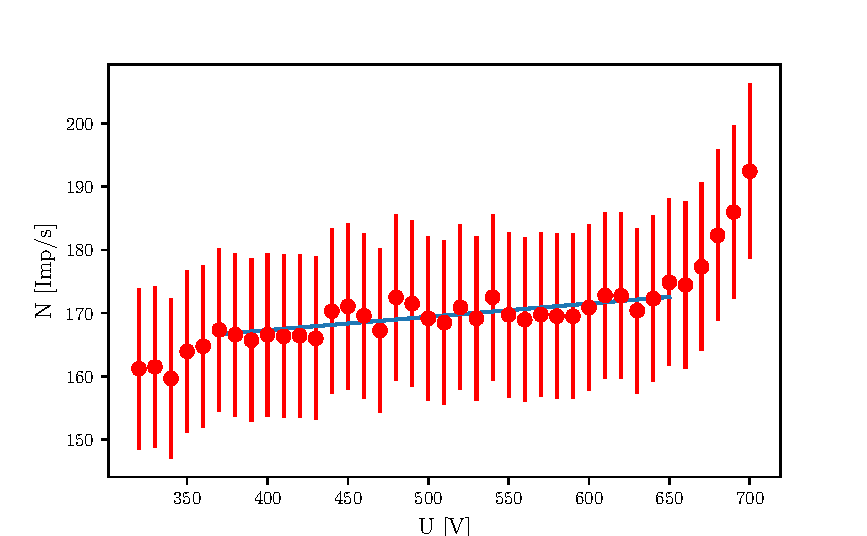
\includegraphics{build/plot.pdf}
    \caption{Anzahl der gemessenen Impulse in Abhängigkeit von der Spannung am Zählrohr}
    \label{fig:plot}
  \end{figure}
  \noindent Das Plateau erstreckt sich circa von $370 $ V bis $640 $ V und wurde mit einer linearen 
  Regression $f = a\cdot U + b$ mit den Koeffizienten $a=1.262 \pm 0.218$ und $b=$ gefittet. 
  Die daraus resultierende Plateau-Steigerung beträgt $1.262 \pm 0.218$ \% pro 100 V. 
  Für einen Reibungslosen Ablauf der folgenden Versuchsteile kann eine Spannung zwischen
  370 V und 640 V gewählt werden.

\subsection{Totzeitbestimmung anhand eines Oszilloskopes}
  Die Zeit zwischen dem ersten und zweiten Puls
  beträgt nach der Momentaufnahme des Oszilloskops
  $T \approx \SI{130}{\mu\second}$.

\subsection{Totzeitbestimmung anhand der Zwei-Quellen-Methode}
  Für die Totzeitbestimmung wurden 120 Sekunden lang zunächst die Impulse $N_1$ einer einzelnen
  $^{204}$Tl-Quelle gemessen, dann die Impulse $N_{1+2}$ von zweien und dann diejenigen der 
  Letzeren. Folgende Werte wurden gemessen:
  \begin{align*}
    N_1     &= 800  \pm 28 \, \text{Imp}/s\\
    N_2     &= 638  \pm 25 \, \text{Imp}/s\\
    N_{1+2} &= 1321 \pm 36 \, \text{Imp}/s\\
  \end{align*}
  Die Totzeit kann näherungsweise durch die in der Theorie hergeleitete Formel 
  \begin{equation*}
  T \approx \dfrac{N_1+N_2-N_{1+2}}{2N_1N_2}= (1,15 \pm 0,47) \cdot 10^{-4} \si{\second}
  \end{equation*}
  bestimmt werden. Die Fehlerfortpflanzung wurde mit Phython Uncertainties berechnet.

\subsection{Berechnung der pro Teilchen freigesetzter Ladungsmenge}
  Es wurde neben der Impulsanzahl in größeren Abständen auch der Zählrohrstrom
  gemessen. Dafür wurden die Werte in Tabelle \ref{fig:Zahlrohrstrom}
  mit einer Genauigkeit von $\Delta I = 0,05 \mu \si{\ampere}$ ermittelt.
  \begin{table}[H]
    \centering
    \caption{Messwerte Zählrohrstrom.}
    \label{fig:Zahlrohrstrom}
    \begin{tabular}{ccc}
    \toprule
    $U [\si{\volt}]$ & $I [\mu\si{\ampere}]$ & $Z [10^{10}]$ \\
    \midrule
    350 & 0,3 & 1,14 \pm 0,21\\
    400	& 0,4 & 1,49 \pm 0,22\\
    450	& 0,7 & 2,55 \pm 0,27\\
    500	& 0,8 & 2,95 \pm 0.29\\
    550	& 1,0 & 3,67 \pm 0,34\\
    600	& 1,3 & 4,74 \pm 0,40\\
    650	& 1,4 & 4,99 \pm 0,42\\
    700	& 1,8 & 5,85 \pm 0,45\\
    \bottomrule
    \end{tabular}
  \end{table}
  \noindent Durch die Beziehung 
  \begin{equation*}
    Z = \dfrac{I \cdot \Delta t}{e_0 \cdot N}
  \end{equation*}
  lässt sich somit die Zahl Z der freigesetzten Ladungen pro eingefallenen Teilchen bestimmen. 
  In der Grafik \ref{fig:plot1} sind die Werte aus Tabelle \ref{fig:Zahlrohrstrom} für die Zahl
  Z auch nochmal graphisch dargestellt.
  \begin{figure}[H]
    \centering
    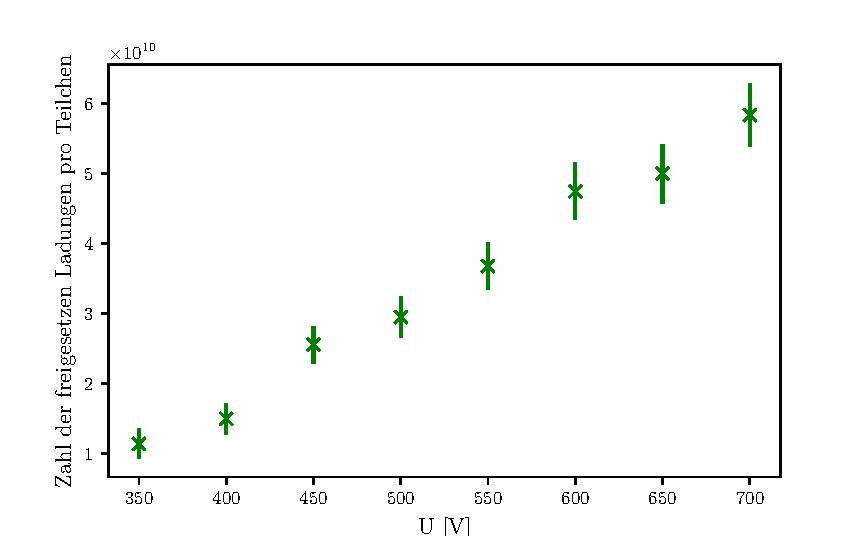
\includegraphics{build/plot1.pdf}
    \caption{Plot.}
    \label{fig:plot1}
  \end{figure}

  \noindent Der Fehler von Z wird anhand der Gaußschen Fehlerfortpflanzung 
  \begin{align*}
    \Delta Z & = Z * \sqrt{\left( \frac{\Delta I}{I} \right)^2 + \left( \frac{\Delta N}{N} \right)^2}\\
  \end{align*}
  bestimmt.